\documentclass[12pt,a4paper]{article}
% math_setup.tex
% Essential Packages
\RequirePackage{etex}
\usepackage{comment}
\usepackage{etex}
\usepackage{listings}
\usepackage{amsmath}    % Advanced math typesetting
\usepackage{amsfonts}   % Math fonts
\usepackage{amssymb}    % Math symbols
\usepackage{amsthm}     % Theorem environment
\usepackage{mathtools}  % More symbols
\usepackage{tikz}       % For drawing diagrams
\usepackage{tikz-network}
\usepackage{pgfplots}
\usetikzlibrary{calc, arrows.meta, positioning, quotes}
\usepackage{mdframed}
\usepackage{float}
\usepackage{thmtools}
\usepackage{xcolor}
\usepackage{geometry}
\usepackage{fancyhdr}
\usepackage[colorlinks=true, linkcolor=blue, citecolor=green, urlcolor=red]{hyperref}
\usepackage{csquotes}
\usepackage[backend=biber, style=ieee]{biblatex}
\pgfplotsset{compat=1.18}
%\usepackage{mdframed}

% Wolfram Code Block
\lstdefinelanguage{Wolfram}{
    keywords={Sum, If, For, While, Do, Plot, Table, Range, Integrate, NIntegrate, D, Solve, NSolve, DSolve, NDSolve, LinearSolve, Expand, Factor, Simplify, FullSimplify, Module, Block, With},
    sensitive=true,
    morecomment=[l]{(*},
    morecomment=[s][\itshape]{(*}{*)},
    morestring=[b]",
    morestring=[b]',
}

\lstset{
    language=Wolfram,
    basicstyle=\ttfamily,
    keywordstyle=\color{blue}\bfseries,
    commentstyle=\color{green}\itshape,
    stringstyle=\color{red},
    showstringspaces=false,
    frame=single,
    breaklines=true,
    numbers=left,
    numberstyle=\tiny\color{gray},
    stepnumber=1,
    numbersep=5pt,
    backgroundcolor=\color{lightgray!20}
}

% add ref
\addbibresource{references.bib}
% Define colors
\definecolor{theoremcolor}{RGB}{230,230,250}  % Light purple
\definecolor{lemmacolor}{RGB}{240,248,255}    % Alice Blue
\definecolor{propcolor}{RGB}{240,255,240}     % Light green
\definecolor{corollarycolor}{RGB}{255,250,240} % Light orange
\definecolor{axiomcolor}{RGB}{255,240,245}    % Lavender blush
\definecolor{definitioncolor}{RGB}{240,255,255} % Light cyan
\definecolor{remarkcolor}{RGB}{245,245,245}   % Light gray
\definecolor{notationcolor}{RGB}{255,250,205}

% Boxed environments

\declaretheoremstyle[
    headfont=\normalfont\bfseries,
    bodyfont=\normalfont,
    headpunct={:},
    postheadspace=1em,
    mdframed={
        linecolor=black,
        backgroundcolor=definitioncolor,
        topline=true,
        bottomline=true,
        leftline=true,
        rightline=true,
        roundcorner=5pt
    }
]{boxeddefinitionstyle}

\declaretheorem[style=boxeddefinitionstyle, name=Definition]{definition}

\declaretheoremstyle[
    headfont=\normalfont\bfseries,
    bodyfont=\normalfont,
    headpunct={:},
    postheadspace=1em,
    mdframed={
        linecolor=black,
        backgroundcolor=theoremcolor,
        topline=true,
        bottomline=true,
        leftline=true,
        rightline=true,
        roundcorner=5pt
    }
]{boxedtheoremstyle}

% Theorem
\declaretheorem[style=boxedtheoremstyle, name=Theorem]{theorem}

% Lemma (adjust color)
\declaretheoremstyle[
    headfont=\normalfont\bfseries,
    bodyfont=\normalfont,
    headpunct={:},
    postheadspace=1em,
    mdframed={
        linecolor=black,
        backgroundcolor=lemmacolor,
        topline=true,
        bottomline=true,
        leftline=true,
        rightline=true,
        roundcorner=5pt
    }
]{boxedlemmastyle}
\declaretheorem[style=boxedlemmastyle, name=Lemma]{lemma}

% Proposition (adjust color)
\declaretheoremstyle[
    headfont=\normalfont\bfseries,
    bodyfont=\normalfont,
    headpunct={:},
    postheadspace=1em,
    mdframed={
        linecolor=black,
        backgroundcolor=propcolor,
        topline=true,
        bottomline=true,
        leftline=true,
        rightline=true,
        roundcorner=5pt
    }
]{boxedpropstyle}
\declaretheorem[style=boxedpropstyle, name=Proposition]{proposition}

% Corollary (adjust color)
\declaretheoremstyle[
    headfont=\normalfont\bfseries,
    bodyfont=\normalfont,
    headpunct={:},
    postheadspace=1em,
    mdframed={
        linecolor=black,
        backgroundcolor=corollarycolor,
        topline=true,
        bottomline=true,
        leftline=true,
        rightline=true,
        roundcorner=5pt
    }
]{boxedcorollarystyle}
\declaretheorem[style=boxedcorollarystyle, name=Corollary]{corollary}

% Axiom (boxed)
\declaretheoremstyle[
    headfont=\normalfont\bfseries,
    bodyfont=\normalfont,
    headpunct={:},
    postheadspace=1em,
    mdframed={
        linecolor=black,
        backgroundcolor=axiomcolor,
        topline=true,
        bottomline=true,
        leftline=true,
        rightline=true,
        roundcorner=5pt
    }
]{boxedaxiomstyle}
\declaretheorem[style=boxedaxiomstyle, name=Axiom]{axiom}

% Remark environment
\declaretheoremstyle[
    headfont=\normalfont\bfseries,
    bodyfont=\normalfont,
    headpunct={:},
    postheadspace=1em,
    mdframed={
        linecolor=black,
        backgroundcolor=remarkcolor,
        topline=true,
        bottomline=true,
        leftline=true,
        rightline=true,
        roundcorner=5pt
    }
]{remarkstyle}
\declaretheorem[style=remarkstyle, name=Remark, numbered=no]{remark}
% Normal, non-italic environments
\declaretheoremstyle[
    headfont=\normalfont\bfseries,
    bodyfont=\normalfont,
    headpunct={:},
    postheadspace=1em,
]{normalstyle}

% Notation environment
\declaretheoremstyle[
    headfont=\normalfont\bfseries,
    bodyfont=\normalfont,
    headpunct={:},
    postheadspace=1em,
    mdframed={
        linecolor=black,
        backgroundcolor=notationcolor,
        topline=true,
        bottomline=true,
        leftline=true,
        rightline=true,
        roundcorner=5pt
    }
]{boxednotationstyle}
\declaretheorem[style=boxednotationstyle, name=Notation]{notation}


% Note environment (more noticeable, with separators, no background, no end symbol)
\newenvironment{note}[1][]
    {\par\vspace{0.5em}\noindent\rule{\textwidth}{0.4pt}\par\vspace{0.5em}%
    \textbf{Note\if\relax\detokenize{#1}\relax\else: #1\fi}\par}
    {\par\vspace{0.5em}\noindent\rule{\textwidth}{0.4pt}\par\vspace{0.5em}}

\declaretheorem[style=normalstyle, name=Note, numbered=no]{oldnote}

\declaretheorem[style=normalstyle, name=Example]{example}
\declaretheorem[style=normalstyle, name=Exercise]{exercise}
\declaretheorem[style=normalstyle, name=Statement]{statement}
\declaretheorem[style=normalstyle, name=Solution, numbered=no]{solution}

% Proof environment (normal, non-italic, with QED symbol)
\declaretheoremstyle[
    headfont=\normalfont\bfseries,
    bodyfont=\normalfont,
    headpunct={:},
    postheadspace=1em,
    qed=$\blacksquare$
]{proofstyle}

\declaretheorem[style=proofstyle, name=Proof]{customproof}

% Shorthand
\newcommand{\vect}[1]{\mathbf{#1}} % For regular vectors
\newcommand{\uvec}[1]{\hat{\mathbf{#1}}} % For unit vectors
\newcommand{\prob}[1]{
    \section*{Problem #1}
}
\newcommand{\R}{\mathbb{R}} % Real numbers
\newcommand{\Z}{\mathbb{Z}} % Integers
\newcommand{\C}{\mathbb{C}} % Complex numbers
\newcommand{\N}{\mathbb{N}} % Natural numbers
\newcommand{\Q}{\mathbb{Q}} % Rational numbers
\newcommand{\Hq}{\mathbb{H}} % Quaternions
\newcommand{\F}{\mathbb{F}} % Finite fields
\newcommand{\Proj}{\mathbb{P}} % Projective space
\newcommand{\K}{\mathbb{K}} % Arbitrary field
\newcommand{\T}{\mathbb{T}} % Torus or sometimes denoted for Topological space
\newcommand{\A}{\mathbb{A}} % Affine space
\newcommand{\0}{\mathbf{0}} % Zero vector
\newcommand{\mbf}[1]{\mathbf{#1}} 
\newcommand{\mat}[1]{\mathbf{#1}}
\newcommand{\adj}{\operatorname{adj}}
\newcommand{\dom}[1]{
    \operatorname{dom}(#1)
}




% Layout
\geometry{a4paper, margin=1in}
\pagestyle{fancy}
\fancyhf{}
\rhead{\today}
\lhead{\textbf{ENG1005 Engineering Mathematics}}
\rfoot{Page \thepage}


\begin{document}
\title{ENG1005 Week3 Workshop Problem Set Solutions}
\author{Yang Xingyu (33533563)}
\date{\today}
\maketitle

\section*{Applied Class Challenges}
\subsection*{Multiplicative Property of Determinant}
\begin{theorem}[Multiplicative Property of Determinant under Matrix Multiplication]
For any \( n \times n \) square matrices \(\mat{A}\) and \(\mat{B}\):
\[
|\mat{A}\mat{B}| = |\mat{A}||\mat{B}|,
\]
and this implies
\[
\adj(\mat{A}\mat{B}) = \adj(\mat{B}) \adj(\mat{A}).
\]
\end{theorem}
\begin{proof}
    Assuming the following proposition is true, we aim to prove Theorem 1.
    \begin{lemma}\label{inv}
      \label{scalarI}  $\forall n \times n$ \textbf{ matrix} \(\mat{A}\), \(\mat{A}\adj(\mat{A})=\adj(\mat{A})\mat{A} =|\mat{A}|\mat{I}\).
    \end{lemma}
    By rearrangement, we have 
    \begin{equation}
    \mat{A}\frac{\adj(\mat{A})}{|\mat{A}|} = \mat{I}
    \end{equation}
    
    Since \(\mat{A}\) is non-singular, then there must exist a unique multiplicative inverse of \(\mat{A}\), which we call \(\mat{A}^{-1}\), such that \(\mat{A}\mat{A}^{-1} = \mat{A}^{-1}\mat{A} = \mat{I}\). Hence, we have
    \begin{equation}
        \frac{\adj(\mat{A})}{|\mat{A}|} = \mat{A}^{-1}
    \end{equation}
A new lemma is needed here to proceed with the proof.
\begin{lemma}
    \label{Inverse_o_Product}If a \textbf{non-singular} matrix \(\mat{A}\) is the product of two other matrices \(\mat{M}\) and \(\mat{N}\), such that \(\mat{A = MN}\), then 
    \[
    \mat{A}^{-1} =  \mat{N}^{-1}\mat{M}^{-1}.
    \]
\end{lemma}
    By Lemma 2 and equation (2), we have 
    \begin{equation}
        \left(\mat{MN}\right)^{-1} = \mat{N}^{-1}\mat{M}^{-1}
    \end{equation}
    Again, by equation (2), we have 
    \begin{equation}
        \mat{N}^{-1} = \frac{\adj(\mat{N})}{|\mat{N}|},  
        \quad \mat{M}^{-1} = \frac{\adj(\mat{M})}{|\mat{M}|}.
    \end{equation}
    Combining equations (3) and (4), we get
    \[
    \left(\mat{MN}\right)^{-1} = \mat{N}^{-1}\mat{M}^{-1} = \frac{\adj(\mat{N})}{|\mat{N}|} \cdot \frac{\adj(\mat{M})}{|\mat{M}|}
    \]
    Therefore, 
    \[
    \left(\mat{MN}\right)^{-1} = \frac{\adj(\mat{MN})}{|\mat{MN}|}
    \]
    Given that \(\left(\mat{MN}\right)^{-1} = \mat{N}^{-1}\mat{M}^{-1}\), we have:
    \[
    \frac{\adj(\mat{MN})}{|\mat{MN}|} = \frac{\adj(\mat{N})}{|\mat{N}|} \cdot \frac{\adj(\mat{M})}{|\mat{M}|}
    \]
    This implies:
    \[
    \adj(\mat{MN}) = \adj(\mat{N}) \adj(\mat{M})
    \]
    and
    \[
    |\mat{A}\mat{B}| = |\mat{A}||\mat{B}|
    \]
    This is because, the structure of the last identity is a fraction on both sides, and the numerator on LHS is a matrix, while a product of matrix on the RHS. The denominator on LHS $|\mat{MN}|\in \F$, and the denominator on RHS is a product of elements in some $\F$. Both the set of all square matrix and any field $\F$ are vector space, and thus the multiplication is closed on their respective set of elements. Hence, we must have the numerator on the LHS is the product of the numerators on RHS, and same goes for the denominator, due to the closure of multiplication under vector space.

    Now we will discuss the case under \textbf{non-singular matrices}.
    When one of or both matrices $\mathbf{A,B}$ are both singular, then the product of the two matrices will still be a singular matrix, as the rank of both original matrices are not of full rank. Thus, in whatever case, we have $0 = 0 \times0$. Hence, the part for determinant is proven, and we may move to the adjugate matrix.

    Considering
    $$
    \begin{cases}
        (\mat{A}\mat{B})\adj(\mat{A}\mat{B}) = |\mat{A}\mat{B}|\mat{I}\\
        \mat{A} \adj(\mat{A}) = |\mat{A}|\mat{I}\\
        \mat{B} \adj(\mat{B}) = |\mat{B}|\mat{I}
    \end{cases}.
    $$
    As long as more than one of the singular matrix $\mat{A,B}$, by what we have previously shown, $|\mat{B}|\mat{I} \cdot |\mat{A}|\mat{I} = |\mat{A}\mat{B}|\mat{I} = \0$. Therefore,
    \[
    (\mat{A}\mat{B})\adj(\mat{A}\mat{B}) = \mat{B} \adj(\mat{B}) \cdot \mat{A} \adj(\mat{A}) = |\mat{BA}|\cdot \mat{I}.
    \]

    Now consider $\mat{A}\mat{B}\adj(\mat{B})\adj(\mat{A})$.
    We have
    \[
    (\mat{A}\mat{B})\adj(\mat{B})\adj(\mat{A}) = \mat{A}(\mat{B}\adj(\mat{B}))\adj(\mat{A})
    =
    |\mat{B}|\mat{I}\cdot \mat{A}\adj(\mat{A}) = |\mat{B}|\mat{I}\cdot |\mat{A}|\mat{I} = |\mat{BA}|\cdot \mat{I}.
    \]
    Hence, $\adj(\mat{A}\mat{B}) = \adj(\mat{B})\adj(\mat{A})$.  We have also proven the case for one or more singular matrix.

    This completes the proof.
\end{proof}
\begin{remark}
    Only when I finished the part discussing case in non-singular matrix and construct $\mat{A}\mat{B}\adj(\mat{B})\adj(\mat{A})$, I realised that this could be used to rewrite the proof without discussing different cases.
\end{remark}
Another approach is using mathematical induction (though I don't really like it). We can prove $|\mat{AB}| = |\mat{A}||\mat{B}|$ and then show that the other statement holds, which is implied by the previous one.

\begin{proof}
We use mathematical induction to prove the previous statement.

Let predicate $P(n)$ to denote that
$$\forall n \times n \text{ square matrix } \mat{A}, \mat{B}, |\mat{A}\mat{B}| = |\mat{A}||\mat{B}|.$$ 
\textbf{Base case ($n = 1$)}

When $n = 1$, we have
\[
\mat{A} = \begin{bmatrix} a \end{bmatrix}, \quad \mat{B} = \begin{bmatrix} b \end{bmatrix}.
\]

So $|\mat{A}\mat{B}| = |\mat{A}||\mat{B}| = ab$, and obviously $P(1)$ holds.

\textbf{Inductive Hypothesis ($n = k$)}

We assume that all $P(k)$ is true. That is, for any $k\times k$ matrix
\[
\mat{A} = \begin{bmatrix}
a_{11} & a_{12} & \dots  & a_{1k} \\
a_{21} & a_{22} & \dots  & a_{2k} \\
\vdots & \vdots & \ddots & \vdots \\
a_{k1} & a_{k2} & \dots  & a_{kk}
\end{bmatrix}, \quad
\mat{B} = \begin{bmatrix}
b_{11} & b_{12} & \dots  & b_{1k} \\
b_{21} & b_{22} & \dots  & b_{2k} \\
\vdots & \vdots & \ddots & \vdots \\
b_{k1} & b_{k2} & \dots  & b_{kk}
\end{bmatrix},
\]

We have
$$|\mat{A}\mat{B}| = |\mat{A}||\mat{B}|.$$


\textbf{Inductive Step ($n = k + 1$)}

Now we need to show that $P(k+1)$ is true. That is, for any two $k+1\times k+1$ matrix
\[
\mat{A} = \begin{bmatrix}
a_{11} & a_{12} & \dots  & a_{1,k+1} \\
a_{21} & a_{22} & \dots  & a_{2,k+1} \\
\vdots & \vdots & \ddots & \vdots \\
a_{k+1,1} & a_{k+1,2} & \dots  & a_{k+1,k+1}
\end{bmatrix}, \quad
\mat{B} = \begin{bmatrix}
b_{11} & b_{12} & \dots  & b_{1,k+1} \\
b_{21} & b_{22} & \dots  & b_{2,k+1} \\
\vdots & \vdots & \ddots & \vdots \\
b_{k+1,1} & b_{k+1,2} & \dots  & b_{k+1,k+1}
\end{bmatrix},
\]
$$|\mat{A}\mat{B}| = |\mat{A}||\mat{B}|.$$

Using Laplace expansion on the first row of the product, we have
\[
|\mat{A} \mat{B}|=\sum_{j=1}^{k+1}(-1)^{1+j}(\mat{A} \mat{B})_{1 j} \mat{M}_{1 j}(\mat{A} \mat{B})
\]

Notice that, every $(\mat{A} \mat{B})_{1 j}$ is the product of the first row of $\mat{A}$ and the $j$-th column of $\mat{B}$:
\begin{equation}\label{w3prodrule}
    (\mat{AB})_{1 j}=\sum_{m=1}^{k+1} \mat{A}_{1 m} \mat{B}_{m j}.
\end{equation}

It is also observed that $\mat{M}_{1 j}(\mat{A} \mat{B})$ is a determinant of $k\times k$ matrix, where our inductive hypothesis is applicable.

So, applying our hypothesis and (\ref{w3prodrule}), we have
\begin{equation}
    |\mat{A} \mat{B}|=\sum_{j=1}^{k+1}(-1)^{1+j}\left(\sum_{m=1}^{k+1} \mat{A}_{1 m} \mat{B}_{m j}\right)
    \mat{M}_{1 j}(\mat{A})\mat{M}_{1 j}(\mat{B})
\end{equation}

By the property of double summation, we have
\[
|\mat{AB}|=
\sum_{j=1}^{k+1} \sum_{m=1}^{k+1} (-1)^{1+j}\mat{A}_{1 m} \mat{B}_{m j}\mat{M}_{1 j}(\mat{A})\mat{M}_{1 j}(\mat{B})
\]

We can again, rearrange the summation, because in this case the subscript $j$ and $m$ have the same lower and upper boundaries. We can split the double summation in to the product of two $k+1$ time summations, and change the subscript variable without changing the result.

\[
|\mathbf{AB}| = 
\sum_{j=1}^{k+1}(-1)^{1+j}\mathbf{A}_{1 j}\mathbf{M}_{1 j}(\mathbf{A})
\sum_{m=1}^{k+1} (-1)^{1+m}\mathbf{B}_{1 m}\mathbf{M}_{1 m}(\mathbf{B})
\]

Note that
\[
|\mathbf{A}| = \sum_{j=1}^{k+1}(-1)^{1+j}\mathbf{A}_{1 j}\mathbf{M}_{1 j}(\mathbf{A}),
\] 
\[
|\mathbf{B}| = \sum_{m=1}^{k+1} (-1)^{1+m}\mathbf{B}_{1 m}\mathbf{M}_{1 m}(\mathbf{B}).
\]

Hence, we have shown that for any two $k+1\times k+1$ matrix, $|\mat{A}\mat{B}| = |\mat{A}||\mat{B}|$, and thus $P(k+1)$ holds.

To sum up, by induction, we have 
\[
P(1) \implies P(2)\implies \cdots \implies P(n),
\]
and the statement is thus proven.
\end{proof}

\subsection*{Geometrical Meaning of Determinant}

\subsubsection*{2D: Area of a Parallelogram in \(\mathbb{R}^2\)}

Consider two vectors \(\mathbf{a} = \begin{bmatrix} a_1 \\ a_2 \end{bmatrix}\) and \(\mathbf{b} = \begin{bmatrix} b_1 \\ b_2 \end{bmatrix}\) in \(\mathbb{R}^2\). These vectors define a parallelogram in the 2D plane. The area \(A\) of this parallelogram can be calculated using the determinant.

The area \(A\) is given by the absolute value of the determinant of the matrix formed by placing \(\mathbf{a}\) and \(\mathbf{b}\) as columns:

\[
A = \left|\begin{vmatrix} a_1 & b_1 \\ a_2 & b_2 \end{vmatrix}\right| = \left|a_1b_2 - a_2b_1\right|
\]

This expression can be expanded as follows:

\[
A = \left| a_1 b_2 - a_2 b_1 \right|
\]

This formula computes the signed area of the parallelogram. The absolute value is taken to ensure the area is positive.

The same area can also be expressed in terms of the magnitudes of the vectors \(\mathbf{a}\) and \(\mathbf{b}\) and the sine of the angle \(\theta\) between them:

\[
A = |\mathbf{a}| |\mathbf{b}| \sin\theta
\]

\begin{remark}
    This is actually how cross product is defined in $\R^2$.
\end{remark}

The determinant captures both the magnitudes of the vectors and the sine of the angle between them, giving the area of the parallelogram. Thus, the determinant in \(\mathbb{R}^2\) can be interpreted as a measure of the area.

\subsubsection*{3D: Volume of a Parallelepiped in \(\mathbb{R}^3\)}

In $\R^3$, consider three vectors:

\[
\mathbf{a} = \begin{bmatrix} a_1 \\ a_2 \\ a_3 \end{bmatrix}, \quad
\mathbf{b} = \begin{bmatrix} b_1 \\ b_2 \\ b_3 \end{bmatrix}, \quad
\mathbf{c} = \begin{bmatrix} c_1 \\ c_2 \\ c_3 \end{bmatrix}
\]

These vectors define a parallelepiped in \(\mathbb{R}^3\). The volume \(V\) of this parallelepiped can be calculated using the determinant.

To compute the volume \(V\) of the parallelepiped defined by \(\mathbf{a}\), \(\mathbf{b}\), and \(\mathbf{c}\), we construct a matrix \(M\) whose columns are these vectors:

\[
M = \begin{bmatrix}
a_1 & b_1 & c_1 \\
a_2 & b_2 & c_2 \\
a_3 & b_3 & c_3
\end{bmatrix}
\]

The volume \(V\) is given by the absolute value of the determinant of \(M\):

\[
V = \left| \det(M) \right| = \left| \begin{vmatrix}
a_1 & b_1 & c_1 \\
a_2 & b_2 & c_2 \\
a_3 & b_3 & c_3
\end{vmatrix} \right|
\]

Expanding the determinant, we have:

\begin{align*}
\det(M) &= a_1 \begin{vmatrix} b_2 & c_2 \\ b_3 & c_3 \end{vmatrix} - b_1 \begin{vmatrix} a_2 & c_2 \\ a_3 & c_3 \end{vmatrix} + c_1 \begin{vmatrix} a_2 & b_2 \\ a_3 & b_3 \end{vmatrix} \\
&= a_1 (b_2 c_3 - b_3 c_2) - b_1 (a_2 c_3 - a_3 c_2) + c_1 (a_2 b_3 - a_3 b_2)
\end{align*}

\begin{remark}
    Anti-intuitively, the volume can be expressed as a linear combination of areas of parallelogram.
\end{remark}
Therefore, the volume is:

\[
V = \left| a_1 (b_2 c_3 - b_3 c_2) - b_1 (a_2 c_3 - a_3 c_2) + c_1 (a_2 b_3 - a_3 b_2) \right|
\]

The scalar triple product offers a geometric interpretation of this determinant. The scalar triple product of vectors \(\mathbf{a}\), \(\mathbf{b}\), and \(\mathbf{c}\) is defined as:

\[
\mathbf{a} \cdot (\mathbf{b} \times \mathbf{c})
\]

This expression computes the volume of the parallelepiped formed by the three vectors. Specifically:

\begin{itemize}
    \item \(\mathbf{b} \times \mathbf{c}\) yields a vector perpendicular to the plane defined by \(\mathbf{b}\) and \(\mathbf{c}\), with magnitude equal to the area of the parallelogram spanned by \(\mathbf{b}\) and \(\mathbf{c}\).
    \item The dot product \(\mathbf{a} \cdot (\mathbf{b} \times \mathbf{c})\) projects \(\mathbf{a}\) onto this perpendicular vector, effectively measuring the component of \(\mathbf{a}\) along the direction perpendicular to the base plane, scaled by the area of the base parallelogram.
\end{itemize}

Thus, the scalar triple product equates to the (signed) volume of the parallelepiped. The sign indicates the orientation (right-handed or left-handed system) of the vectors.

Mathematically:

\[
V = \left| \mathbf{a} \cdot (\mathbf{b} \times \mathbf{c}) \right|
\]

To show that this is equivalent to the determinant computed earlier, we can express the scalar triple product in terms of the components of the vectors:

\[
\mathbf{a} \cdot (\mathbf{b} \times \mathbf{c}) = \begin{bmatrix} a_1 \\ a_2 \\ a_3 \end{bmatrix} \cdot \left( \begin{bmatrix} b_2 c_3 - b_3 c_2 \\ b_3 c_1 - b_1 c_3 \\ b_1 c_2 - b_2 c_1 \end{bmatrix} \right ) = a_1 (b_2 c_3 - b_3 c_2) + a_2 (b_3 c_1 - b_1 c_3) + a_3 (b_1 c_2 - b_2 c_1)
\]

Notice that this expression matches the expanded determinant of matrix \(M\) obtained earlier. Therefore:

\[
V = \left| \mathbf{a} \cdot (\mathbf{b} \times \mathbf{c}) \right| = \left| \det(M) \right|
\]
\subsubsection*{4D and Beyond: Hypervolume in Higher Dimensions}

In higher dimensions, the concept of volume generalizes to hypervolume. Consider \(n\) vectors \(\mathbf{v}_1, \mathbf{v}_2, \dots, \mathbf{v}_n\) in \(\mathbb{R}^n\). These vectors define a parallelepiped in \(n\)-dimensional space. The hypervolume \(H\) of this parallelepiped is given by the absolute value of the determinant:

\[
H = \left|\det\begin{bmatrix} 
v_{11} & v_{12} & \dots & v_{1n} \\
v_{21} & v_{22} & \dots & v_{2n} \\
\vdots & \vdots & \ddots & \vdots \\
v_{n1} & v_{n2} & \dots & v_{nn}
\end{bmatrix}\right|
\]

This determinant represents the signed hypervolume of the parallelepiped, generalizing the concept of volume to higher dimensions. The sign indicates the orientation of the vectors in the \(n\)-dimensional space.


\section*{Problem 1}
\begin{solution}
By substituting $(1,6), (2,7),(3,5)$ to
\begin{equation}
\label{givenw3}
y(x)= Ax^2+B x+C,
\end{equation}
we have 
$$\begin{cases}
A + B + C = 6\\
4A + 2B + C = 7\\
9A + 3B + C = 5
\end{cases}.
$$

In matrix, that is:
\[
\begin{bmatrix}
1 & 1 & 1 \\
4 & 2 & 1 \\
9 & 3 & 1
\end{bmatrix}
\begin{bmatrix}
A \\
B \\
C
\end{bmatrix}
=
\begin{bmatrix}
6 \\
7 \\
5
\end{bmatrix}.
\]
\end{solution}


\section*{Problem 2}
\begin{solution}
Rewrite the system into coefficient matrix $\mat{A}$, we have
\begin{equation}\label{mat1}
\mat{A}=
\left[
\begin{array}{ccc}
1 & 1 & 1 \\
4 & 2 & 1 \\
9 & 3 & 1 
\end{array}
\right].
\end{equation}
We use the Laplace expansion to calculate the determinant.
\begin{definition}
    For an \(n \times n\) matrix \(\mat{B}\), the determinant \(\det(\mat{B})\) can be expanded along any row or column. The formula is:

\[
\det(\mat{B}) = \sum_{j=1}^{n} (-1)^{i+j} b_{ij} \det(\mat{B}_{ij})
\]

where \(b_{ij}\) is the element of matrix \(\mat{B}\) at row \(i\) and column \(j\), and \(\mat{B}_{ij}\) is the \((n-1) \times (n-1)\) submatrix obtained by deleting the \(i\)-th row and \(j\)-th column of \(\mat{B}\).
\end{definition}
$\det(\mat{A}) = $
We choose to expand along the first row of the matrix \(\mat{A}\):

\[
\mat{A}=
\left[
\begin{array}{ccc}
1 & 1 & 1 \\
4 & 2 & 1 \\
9 & 3 & 1
\end{array}
\right].
\]

Calculating the determinant \(\det(\mat{A})\):

\[
\det(\mat{A}) = 1 \cdot 
\begin{vmatrix}
2 & 1 \\
3 & 1
\end{vmatrix}
- 1 \cdot 
\begin{vmatrix}
4 & 1 \\
9 & 1
\end{vmatrix}
+ 1 \cdot 
\begin{vmatrix}
4 & 2 \\
9 & 3
\end{vmatrix}
\]

where,

\[
\begin{vmatrix}
2 & 1 \\
3 & 1
\end{vmatrix}
= 2 \cdot 1 - 1 \cdot 3 = 2 - 3 = -1
\]

\[
\begin{vmatrix}
4 & 1 \\
9 & 1
\end{vmatrix}
= 4 \cdot 1 - 1 \cdot 9 = 4 - 9 = -5
\]

\[
\begin{vmatrix}
4 & 2 \\
9 & 3
\end{vmatrix}
= 4 \cdot 3 - 2 \cdot 9 = 12 - 18 = -6
\]

Substituting these into the formula:

\[
\det(\mat{A}) = 1 \cdot (-1) - 1 \cdot (-5) + 1 \cdot (-6) = -1 + 5 - 6 = -2
\]

Therefore, the determinant of matrix \(\mat{A}\) is $\det(\mat{A}) = -2$.

This tells us that the system is solvable and has specific solution, so we can make sure we will find a unique curve to fit the trajectory.
\end{solution}


\section*{Problem 3}
\begin{solution}
By lemma \ref{inv}, we have
\[
\mat{A}^{-1} = \frac{\adj(\mat{A})}{|\mat{A}|}.
\]

So to get  $\mat{A}^{-1}$, we only need to find $\adj(\mat{A})$.

We know that $\adj(\mat{A}) = \mat{C}^T$, where $\mat{C}$ is the cofactor matrix of $\mat{A}$. Each element in $\mat{C}$ is given by
$$
C_{i j}=(-1)^{i+j} M_{i j},
$$
where $M_{i j}$ is the determinant of the $(n-1) \times(n-1)$ submatrix obtained by deleting the $i$-th row and $j$-th column of $\mathbf{A}$.

After calculation, we have 
\[
\adj(\mat{A})=
\left(
\begin{array}{ccc}
 \left| 
\begin{array}{cc}
 2 & 1 \\
 3 & 1 \\
\end{array}
\right|  & \left| 
\begin{array}{cc}
 1 & 1 \\
 1 & 3 \\
\end{array}
\right|  & \left| 
\begin{array}{cc}
 1 & 1 \\
 2 & 1 \\
\end{array}
\right|  \\ \\
 \left| 
\begin{array}{cc}
 1 & 4 \\
 1 & 9 \\
\end{array}
\right|  & \left| 
\begin{array}{cc}
 1 & 1 \\
 9 & 1 \\
\end{array}
\right|  & \left| 
\begin{array}{cc}
 1 & 1 \\
 1 & 4 \\
\end{array}
\right|  \\ \\
 \left| 
\begin{array}{cc}
 4 & 2 \\
 9 & 3 \\
\end{array}
\right|  & \left| 
\begin{array}{cc}
 1 & 1 \\
 3 & 9 \\
\end{array}
\right|  & \left| 
\begin{array}{cc}
 1 & 1 \\
 4 & 2 \\
\end{array}
\right|  \\
\end{array}
\right),
\]

and thus, we have 
\[
\mat{A}^{-1} = -\frac{1}{2} 
\left[
\begin{array}{ccc}
 -1 & 2 & -1 \\
 5 & -8 & 3 \\
 -6 & 6 & -2 \\
\end{array}
\right]
=
\left[
\begin{array}{ccc}
 \frac{1}{2} & -1 & \frac{1}{2} \\
 -\frac{5}{2} & 4 & -\frac{3}{2} \\
 3 & -3 & 1 \\
\end{array}
\right].
\]
\begin{remark}
An alternative way here is Gauss-Jordan Elimination. We can apply Gaussian elimination with an identity matrix simultaneously, and when we have the matrix on the left an identity matrix, we will have its inverse matrix on the right.
\[
\left[
\begin{array}{ccc|ccc}
 1 & 1 & 1 & 1 & 0 & 0 \\
 4 & 2 & 1 & 0 & 1 & 0 \\
 9 & 3 & 1 & 0 & 0 & 1 \\
\end{array}
\right]
\]
\begin{center}
$R_2 \leftarrow R_2 - 4\times R_1$
\[
\left[
\begin{array}{ccc|ccc}
 1 & 1 & 1 & 1 & 0 & 0 \\
 0 & -2 & -3 & -4 & 1 & 0 \\
 9 & 3 & 1 & 0 & 0 & 1 \\
\end{array}
\right]
\]
$R_3 \leftarrow R_3 - 9\times R_1$
\[
\left[
\begin{array}{ccc|ccc}
 1 & 1 & 1 & 1 & 0 & 0 \\
 0 & -2 & -3 & -4 & 1 & 0 \\
 0 & -6 & -8 & -9 & 0 & 1 \\
\end{array}
\right]
\]
$R_2 \leftrightarrow R_3$
\[
\left[
\begin{array}{ccc|ccc}
 1 & 1 & 1 & 1 & 0 & 0 \\
 0 & -6 & -8 & -9 & 0 & 1 \\
 0 & -2 & -3 & -4 & 1 & 0 \\
\end{array}
\right]
\]
$R_3 \leftarrow R_3 - \frac{1}{3} R_2$
\[
\left[
\begin{array}{ccc|ccc}
 1 & 1 & 1 & 1 & 0 & 0 \\
 0 & -6 & -8 & -9 & 0 & 1 \\
 0 & 0 & -\frac{1}{3} & -1 & 1 & -\frac{1}{3} \\
\end{array}
\right]
\]
$R_3 \leftarrow -3 \times R_3$
\[
\left[
\begin{array}{ccc|ccc}
 1 & 1 & 1 & 1 & 0 & 0 \\
 0 & -6 & -8 & -9 & 0 & 1 \\
 0 & 0 & 1 & 3 & -3 & 1 \\
\end{array}
\right]
\]
$R_2 \leftarrow R_2 + 8\times R_3$
\[
\left[
\begin{array}{ccc|ccc}
 1 & 1 & 1 & 1 & 0 & 0 \\
 0 & -6 & 0 & 15 & -24 & 9 \\
 0 & 0 & 1 & 3 & -3 & 1 \\
\end{array}
\right]
\]
$R_2 \leftarrow -\frac{1}{6}\times R_2$
\[
\left[
\begin{array}{ccc|ccc}
 1 & 1 & 1 & 1 & 0 & 0 \\
 0 & 1 & 0 & -\frac{5}{2} & 4 & -\frac{3}{2} \\
 0 & 0 & 1 & 3 & -3 & 1 \\
\end{array}
\right]
\]
$R_1 \leftarrow R_1 - R_2 - R_3$
\[
\left[
\begin{array}{ccc|ccc}
 1 & 0 & 0 & \frac{1}{2} & -1 & \frac{1}{2} \\
 0 & 1 & 0 & -\frac{5}{2} & 4 & -\frac{3}{2} \\
 0 & 0 & 1 & 3 & -3 & 1 \\
\end{array}
\right]
\]
\end{center}

So $\mat{A}^{-1} = 
\left[
\begin{array}{ccc}
 \frac{1}{2} & -1 & \frac{1}{2} \\
 -\frac{5}{2} & 4 & -\frac{3}{2} \\
 3 & -3 & 1 \\
\end{array}
\right]
$.

\end{remark}

The system can be written as
\[
\mat{A}
\cdot
\begin{bmatrix}
    A\\B\\C
\end{bmatrix}
=
\begin{bmatrix}
    6\\7\\5
\end{bmatrix}
\]
Since $\mat{A}^{-1}$ has the same dimension as $\mat{A}$, we can left multiply $\mat{A}^{-1}$ on both sides, so we have
\[
\mat{A}^{-1}
\cdot
\mat{A}
\cdot
\begin{bmatrix}
    A\\B\\C
\end{bmatrix}
=
\mat{A}^{-1}
\cdot
\begin{bmatrix}
    6\\7\\5
\end{bmatrix}
\implies
\begin{bmatrix}
    A\\B\\C
\end{bmatrix}
=
\mat{A}^{-1}
\cdot
\begin{bmatrix}
    6\\7\\5
\end{bmatrix}
\]
So,
\[
\begin{bmatrix}
    A\\B\\C
\end{bmatrix}
=
\begin{bmatrix}
    \frac{1}{2}\times 6 - 7 + \frac{1}{2}\times 5\\
    -\frac{5}{2}\times 6  + 4 \times 7 - \frac{3}{2}\times 5\\
    3\times 6 - 3\times 7 + 5
\end{bmatrix}
= 
\begin{bmatrix}
    -\frac{3}{2}\\
    \frac{11}{2}\\
    2
\end{bmatrix}.
\]
Hence, the solution is 
$\begin{cases}
    A = -\frac{3}{2}\\
    B =  \frac{11}{2}\\
    C = 2
\end{cases}$
\end{solution}

\section*{Problem 4}
Substitute 
$\begin{cases}
    A = -\frac{3}{2}\\
    B =  \frac{11}{2}\\
    C = 2
\end{cases}$
to (\ref{givenw3}), we have 
\[
y(x) = -\frac{3}{2}x^2 + \frac{11}{2}x + 2
\]
The missile lands when $y(x) = 0$. To get the position when $y(x) = 0$, we only need to solve the quadratic equation:
\[
-\frac{3}{2}x^2 + \frac{11}{2}x + 2 = 0 \equiv -3x^2 + 11x + 4 = 0
\]

This can be factorised to
\[
(x-4)(-3 x-1)=0
\]
Hence, $x = 4$ or $x = -\frac{1}{3}$, the latter does not make sense here, since the the missile is launched at where $x = 0$.
So, it lands when it is 4 units away from the origin.






\section*{Problem 5}
\begin{solution}
Yes, we can find a unique trajectory function for the object. 

This is because it requires only four unknowns to identify the function, and we are provided four points on the function. 

If we substitute these points into the expression respectively, we will get a system of linear equation, whose coefficient matrices satisfies all row vectors are independent from each other. So, the augmented matrix $(A|b)$ satisfies $rank(A)=rank(b) = n$, where $n$ is the number of unknowns.

Therefore, by Rouché-Capelli Theorem, we can find a specific solution for the system of linear equations, so that a unique cubic function can be identified.
\end{solution}

\section*{problem 6}
\begin{solution}
    By substituting the points into the relation, we have
    \begin{equation}\label{w3cubiccoe}
        \mat{D} = \begin{cases}
            A + B + C + D = 6\\
            8A + 4B + 2C + D = 7\\
            27A + 9B + 3C + D = 5\\
            64A + 16B + 4C + D = 4
        \end{cases}
    \end{equation}
    In matrix, we have
    \[
\begin{bmatrix}
1 & 1 & 1 & 1 \\
8 & 4 & 2 & 1 \\
27 & 9 & 3 & 1 \\
64 & 16 & 4 & 1
\end{bmatrix}
\begin{bmatrix}
A \\
B \\
C \\
D
\end{bmatrix}
=
\begin{bmatrix}
6 \\
7 \\
5 \\
4
\end{bmatrix}.
\]

\section*{Problem 7}
This matrix has a very interesting property, which could help us simplify the calculation of \(|\mat{D}|\).
We can exchange column 1 and column 4, and then exchange column 2 and column 3. This will not change the determinant, since we exchanged it twice, \( -(-|\mat{D}|) = |\mat{D}| \).

The exchange makes
\[
\mat{D} = 
\begin{bmatrix}
1 & 1 & 1 & 1 \\
1 & 2 & 4 & 8 \\
1 & 3 & 9 & 27 \\
1 & 4 & 16 & 64
\end{bmatrix}.
\]

This allows us to identify the matrix as a Vandermonde matrix, whose determinant can be obtained by \( \prod_{0 \leq i < j \leq n} (x_j - x_i) \), and \( n = 4 \) in this case.

So we have 
\[
\det(\mat{D}) = \prod_{0 \leq i < j \leq 4} (x_j - x_i) = (4-3) \times (4-2) \times (4-1) \times (3-2) \times (3-1) \times (2-1) = 12.
\]

This means we can find a unique function through the four data points, since it's a non-singular matrix, \(\det(\mat{D}) \neq 0\).

\begin{remark}
Here we attach the proof of the determinant \parencite{kalman_generalized_1984, rushanan_vandermonde_1989}.
\begin{definition}[Vandermonde Matrix]
    A Vandermonde matrix is an \((m+1) \times (n+1)\) matrix \(\mat{V}\) such that:
    $$
    \mat{V}=
    \begin{bmatrix}
    1 & x_0 & x_0^2 & \ldots & x_0^n \\
    1 & x_1 & x_1^2 & \ldots & x_1^n \\
    1 & x_2 & x_2^2 & \ldots & x_2^n \\
    \vdots & \vdots & \vdots & \ddots & \vdots \\
    1 & x_m & x_m^2 & \ldots & x_m^n
    \end{bmatrix}.
    $$
\end{definition}
The Vandermonde matrix is widely used in the interpolation of polynomials, and in this case of finding coefficients, we must have a square matrix. The following rule is very useful in finding the determinant of a Vandermonde matrix.
\begin{corollary}
    When \(m = n\), the Vandermonde matrix is square, and its determinant has a special form. The determinant of a square Vandermonde matrix \(\mat{V}\) of size \((n+1) \times (n+1)\) is given by:

\[
\det(\mat{V}) = \prod_{0 \leq i < j \leq n} (x_j - x_i).
\]
\end{corollary}
\begin{proof}
By iterating through each column of the matrix, from right to left, until we reach the first column (we will not do anything to it). We will subtract the value on the previous column (on the left) multiplied by \(x_0\), from the current elements. This will make the first row (except the first entry) 0, and the rest of the rows (each) will have common factor \((x_i - x_0), 1 \leq i \leq n\).

$$
\mat{V}=\left[\begin{array}{cccccc}
1 & 0 & 0 & 0 & \cdots & 0 \\
1 & x_1-x_0 & x_1\left(x_1-x_0\right) & x_1^2\left(x_1-x_0\right) & \cdots & x_1^{n-1}\left(x_1-x_0\right) \\
1 & x_2-x_0 & x_2\left(x_2-x_0\right) & x_2^2\left(x_2-x_0\right) & \cdots & x_2^{n-1}\left(x_2-x_0\right) \\
\vdots & \vdots & \vdots & \vdots & \ddots & \vdots \\
1 & x_n-x_0 & x_n\left(x_n-x_0\right) & x_n^2\left(x_n-x_0\right) & \cdots & x_n^{n-1}\left(x_n-x_0\right)
\end{array}\right]
$$

If we measure \(\det(\mat{V})\) using Laplace expansion, we will find that \(\det(\mat{V}) = \det(\mat{M})\), where
\[
\mat{M}=\left[\begin{array}{ccccc}
x_1-x_0 & x_1\left(x_1-x_0\right) & x_1^2\left(x_1-x_0\right) & \cdots & x_1^{n-1}\left(x_1-x_0\right) \\
x_2-x_0 & x_2\left(x_2-x_0\right) & x_2^2\left(x_2-x_0\right) & \cdots & x_2^{n-1}\left(x_2-x_0\right) \\
\vdots & \vdots & \vdots & \ddots & \vdots \\
x_n-x_0 & x_n\left(x_n-x_0\right) & x_n^2\left(x_n-x_0\right) & \cdots & x_n^{n-1}\left(x_n-x_0\right)
\end{array}\right].
\]

Since each row has common factors, we can just take it outside as a scalar when we deal with its determinant. So we have,
\[
\operatorname{det}(\mat{V})=\left(x_1-x_0\right)\left(x_2-x_0\right) \cdots\left(x_n-x_0\right)\left|\begin{array}{ccccc}
1 & x_1 & x_1^2 & \cdots & x_1^{n-1} \\
1 & x_2 & x_2^2 & \cdots & x_2^{n-1} \\
\vdots & \vdots & \vdots & \ddots & \vdots \\
1 & x_n & x_n^2 & \cdots & x_n^{n-1}
\end{array}\right|
\]
\[
=\prod_{1 \leq i \leq n}\left(x_i-x_0\right) \operatorname{det}\left(\mat{V}^{\prime}\right)
\]

It is observed that \(\mat{V}^{\prime}\) is also a Vandermonde matrix, so we can apply the same algorithm again.

The execution of the algorithm comes to an end when \(\mat{V}^{\prime}\) is a \(1 \times 1\) square matrix with 1 as the only entry. Then, we will get all possible permutations of differences between elements in column two \(x_i, x_j\), where \(j > i\).

Hence, we can deduce that
\[
\det(\mat{V})=\prod_{0 \leq i < j \leq n}(x_j - x_i).
\]
\end{proof}
\begin{note}
    The proof maybe not very exhaustive and rigorous, but is enough to show how its determinant works.
\end{note}
\end{remark}
\end{solution}

\section*{Problem 8}
\begin{solution}
Use the following wolfram code,
\begin{lstlisting}
m = {{1, 1, 1, 1}, {8, 4, 2, 1}, {27, 9, 3, 1}, {64, 16, 4, 1}};
b = {6, 7, 5, 4};
x = LinearSolve[m, b]
\end{lstlisting}

we get the solution for (\ref{w3cubiccoe}):
$$
A=\frac{2}{3}, \quad B=-\frac{11}{2}, \quad C=\frac{77}{6}, \quad D=-2 .
$$
\end{solution}
\section*{Problem 9}
\begin{solution}
By substituting the solutions into the polynomial, we have
\[
y(x) = \frac{2}{3}x^3 -\frac{11}{2}x^2 + \frac{77}{6}x -2.
\]

We draw $y(x)$ using tikz and pgfplots below.

\begin{figure}[H]
    \centering
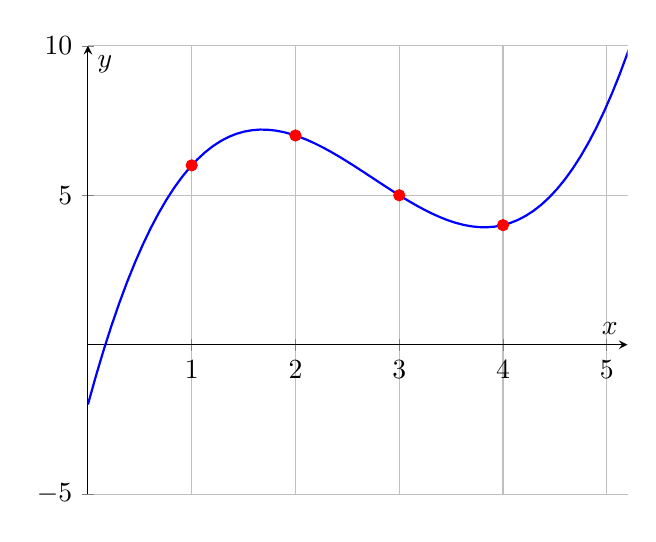
\begin{tikzpicture}
  \begin{axis}[
    axis lines = middle,
    xlabel = \(x\),
    ylabel = \(y\),
    domain = 0:15, 
    samples = 200,
    grid = both,
    legend pos = north west,
    ymin = -5,
    ymax = 10
  ]
    \addplot[
      blue, 
      thick
    ] {2/3 * x^3 - 11/2 * x^2 + 77/6 * x - 2};
    
    
    \addplot[
      only marks,
      red,
      mark = *,
      mark size = 2pt
    ] coordinates {
      (1, 6)
      (2, 7)
      (3, 5)
      (4, 4)
    };
    

  \end{axis}
\end{tikzpicture}

    \caption{$y(x) = \frac{2}{3}x^3 -\frac{11}{2}x^2 + \frac{77}{6}x -2$}
    \label{w3cubgraph}
\end{figure}
\end{solution}

\section*{Problem 10}
\begin{solution}
    The missile will never land. If we assume that this missile will must hit its target at some point $(x, 0)$, then this will not happen. Because the value of $y(x)$ keeps increasing after it reaches its second stationary point $(4,4)$. However, if the missile is set to be very agile and are trying to hit a target in the air that is not far away from where it is launched, then this graph could make sense.


\end{solution}
\section*{Problem 11}
\begin{solution}
The three points are not colinear. If we suppose they are colinear, then any two direction vector between the any of two points chosen will be the same. However, $(2,7)-(1,6) = (1,1)$, while $(3,5)-(2,7) = (1,-2)$. Hence do not lie on a straight line.
\end{solution}

\section*{Problem 12}
By substituting the predicted values into the relation, we have
\begin{solution}
\[
\begin{cases}
    S + T = y(1)\\
    2S + T = y(2)\\
    3S + T = y(3)
\end{cases}.
\]
\end{solution}

\section*{Problem 13}
\begin{solution}
The system can be written as:
\[
\begin{bmatrix}
y(1) \\
y(2) \\
y(3)
\end{bmatrix}
=
S \begin{bmatrix}
1 \\
2 \\
3
\end{bmatrix}
+
T \begin{bmatrix}
1 \\
1 \\
1
\end{bmatrix}
\]

To make it clearer, we can add $\0$ to the RHS.
\[
\begin{bmatrix}
y(1) \\
y(2) \\
y(3)
\end{bmatrix}
=
\begin{bmatrix}
0 \\
0 \\
0
\end{bmatrix}
+
S \begin{bmatrix}
1 \\
2 \\
3
\end{bmatrix}
+
T \begin{bmatrix}
1 \\
1 \\
1
\end{bmatrix}
\]

We first focus on the RHS. The expression on the right can be interpreted as creating a new plane from the origin in $\R^3$ using two column vectors scaled by some parameter $S$ and $T$ respectively. From the size of the column vector, we know they are vectors in $\R^3$.

From the LHS, we know that the result of the linear transformation on the right will create a new point in $\R^3$, combining this to what we derived earlier, we can confirm that
\[
\exists \alpha \subseteq \R^3, \forall S, T \in \R, 
\begin{bmatrix}
    S + T\\ 2S + T\\ 3S+T
\end{bmatrix}
\in \alpha.
\]
\end{solution}

\section*{Problem 14}
\begin{solution}
    To find the minimum distance, between $(6,7,5)$ and the plane, we simply need to find the projection of some direction vector between a point on the plane and the actual coordinate on the normal to the plane.

    We already know that 
    $
    \begin{bmatrix}
1 \\
2 \\
3
\end{bmatrix}$
and 
$\begin{bmatrix}
1 \\
1 \\
1
\end{bmatrix}$
are two direction vectors on the solution plane, so we can find a normal vector to the plane (call $\alpha$):
\[
\vec{n} = \begin{bmatrix}
1 \\
2 \\
3
\end{bmatrix}
\times
\begin{bmatrix}
1 \\
1 \\
1
\end{bmatrix}
=
\begin{bmatrix}
-1 \\
2 \\
-1
\end{bmatrix}
\]

From earlier, we know that 
$\begin{bmatrix}
    0\\0\\0
\end{bmatrix}\in \alpha$, 
so we have a direction vector from the plane to actual coordinate, we call $\vec{v}$:
\[
\vec{v} = 
\begin{bmatrix}
    6\\7\\5
\end{bmatrix}
-
\begin{bmatrix}
    0\\0\\0
\end{bmatrix}
=
\begin{bmatrix}
    6\\7\\5
\end{bmatrix}
\]
\end{solution}

Now we can calculate the minimum distance $d$ as projection of $\vec{v} \text{ on } \vec{n}$.
\[
d = \frac{|\vec{v}\cdot \vec{n}|}{|\vec{n}|} 
= \frac{|6\times(-1) + 7 \times 2 + 5\times (-1)|}{\sqrt{6}}
= \frac{|-6+14-5|}{\sqrt{6}} = \frac{\sqrt{6}}{2}
\]

\section*{Problem 15}
\begin{solution}
    We can find the optimised line by least squares method.
    \[
    S=\frac{N \sum x y-\sum x \sum y}{N \sum x^2-\left(\sum x\right)^2}, 
    \text{     }
    T=\frac{\sum y-S \sum x}{N}
    \]
We have
$$
S=\frac{3 \times 35-6 \times 18}{3 \times 14-6^2}=\frac{105-108}{42-36}=\frac{-3}{6}=-\frac{1}{2}
$$
and
$$
T=\frac{18-\left(-\frac{1}{2}\right) \times 6}{3}=\frac{18+3}{3}=\frac{21}{3}=7
$$

So the optimised line is $f(x) = -\frac{1}{2}x + 7$.

\begin{remark}
We may show how it works (only for the linear function, because I do not know much about vector calculus, hope I'll learn that soon in ENG2005).

The idea here is basically to minimise the difference between the predicted value by the model (the function here).

If we compare the difference between our prediction and real value for the same $x$ one by one, we can define something called the loss (function) of the model, like
\[
loss(S,T) = \sum_{i=1}^n(y_i-f(x)) = \sum_{i=1}^n[y_i- (Sx_i + T)]
\]
where
\begin{itemize}
    \item $n$ is the number of samples.
    \item $x_i, y_i$ are the $i$th $x$ value and actual value respectively.
    \item $S, T$ are the parameters introduced in the problem.
\end{itemize}

But in real practice, we tend to square the difference, as sum up everything directly can sometimes cause confusion, for example, when we have some negative and positive terms that offset each other. Also we are doing this to make sure all errors can be measured by a positive value. Additionally, we use the mean of the squared sum to measure the disparity to make sure each sample has equal contribution to the total loss (\cite{zhou_machine_2021}). Therefore, we define the most common mean square loss function, in this case, as
\[
loss(S,T) = \frac{1}{n}\sum_{i=1}^n[y_i- (Sx_i + T)]^2.
\]

The principal goal of linear regression is basically minimise the value of the function. But we can just rule out the constant coefficient before the summation, as it does not affect the optimisation, since $\frac{1}{n} > 0$. So actually, we only need to minimise 
\[
g(S, T) = \sum_{i=1}^n[y_i- (Sx_i + T)]^2.
\]

This makes it clear its geometrical meaning. We see that this function add up the squared Euclidean distances between each predicted data and actual data.

We can get $\min(g(S,T))$ by taking partial derivatives on $S$ and $T$ respectively, since this function is a binary quadratic function, meaning that we have an extreme value when the value of derivative functions equals zero.

First, we take the partial derivative of $g(S, T)$ with respect to $T$:

\[
\frac{\partial g(S, T)}{\partial T} = \frac{\partial}{\partial T} \sum_{i=1}^{n} \left[ y_i - Sx_i - T \right]^2
\]

Expanding using the chain rule:

\[
\frac{\partial g(S, T)}{\partial T} = -2 \sum_{i=1}^{n} \left[ y_i - Sx_i - T \right]
\]

Setting the derivative to zero gives:

\[
\sum_{i=1}^{n} \left[ y_i - Sx_i - T \right] = 0
\]

which can be rearranged to:

\[
\sum_{i=1}^{n} y_i = S \sum_{i=1}^{n} x_i + n T
\]

Thus, the intercept $T$ is:

\[
T = \frac{\sum_{i=1}^{n} y_i - S \sum_{i=1}^{n} x_i}{n}
\]

Next, we take the partial derivative of $g(S, T)$ with respect to $S$:

\[
\frac{\partial g(S, T)}{\partial S} = \frac{\partial}{\partial S} \sum_{i=1}^{n} \left[ y_i - Sx_i - T \right]^2
\]

Again, expanding using the chain rule:

\[
\frac{\partial g(S, T)}{\partial S} = -2 \sum_{i=1}^{n} x_i \left[ y_i - Sx_i - T \right]
\]

Setting the derivative to zero gives:

\[
\sum_{i=1}^{n} x_i y_i = S \sum_{i=1}^{n} x_i^2 + T \sum_{i=1}^{n} x_i
\]

Substituting the expression for $T$ from the previous step, and simplifying, we obtain the formula for the slope $S$:

\[
S = \frac{n \sum_{i=1}^{n} x_i y_i - \sum_{i=1}^{n} x_i \sum_{i=1}^{n} y_i}{n \sum_{i=1}^{n} x_i^2 - \left( \sum_{i=1}^{n} x_i \right)^2}
\]

So that's how we derive the formula for this basic case.

\end{remark}
\end{solution}

\printbibliography
\end{document}